\documentclass[a4paper,10pt,twocolumn]{ltjsarticle}
\usepackage[haranoaji]{luatexja-preset}
\usepackage[top=18mm,bottom=20mm,left=17mm,right=17mm,columnsep=8mm]{geometry}
\usepackage{graphicx,booktabs,array,caption,enumitem,xcolor,tikz}
\usetikzlibrary{shapes.geometric}
\setlength{\parindent}{1\zw}
\renewcommand{\baselinestretch}{1.0}
\setlength{\parskip}{0pt}
\renewcommand{\thesection}{\arabic{section}.}
\renewcommand{\thesubsection}{\arabic{section}.\arabic{subsection}.}
\makeatletter
\renewcommand{\section}{\@startsection{section}{1}{\z@}{1.1\Cvs \@plus.4\Cdp \@minus.2\Cdp}{.5\Cvs \@plus.2\Cdp}{\normalfont\gtfamily\bfseries\large}}
\renewcommand{\subsection}{\@startsection{subsection}{2}{\z@}{.8\Cvs \@plus.3\Cdp \@minus.2\Cdp}{.3\Cvs \@plus.1\Cdp}{\normalfont\gtfamily\bfseries\normalsize}}
\makeatother
\captionsetup{font={small,sf},labelsep=space,justification=raggedright,singlelinecheck=false,skip=3pt}
\captionsetup[table]{position=top}
\setlist[itemize]{leftmargin=1.2\zw,itemsep=0pt,topsep=2pt,parsep=0pt}
\setlength{\textfloatsep}{8pt plus 2pt minus 2pt}
\setlength{\floatsep}{8pt plus 2pt minus 2pt}
\setlength{\intextsep}{8pt plus 2pt minus 2pt}
\pagestyle{plain}
\raggedbottom
\begin{document}
\twocolumn[{
\noindent\fbox{\gtfamily\small\ 生成AI論文\ }\par\medskip
\begin{center}
{\gtfamily\bfseries\LARGE 免許を持つ人が教えていない：高校情報科の担当者の配置を自治体別に見る$^{\dagger}$}\par\medskip
{\gtfamily\bfseries\large 免許状のない担当者と，免許状を持つが担当していない者の自治体別の関係（令和4年5月1日現在）}\par\medskip
{\normalsize EduData調査研究グループ$^{*1}$・教育データサイエンス解析班$^{*2}$}\par
{\small オープン教育統計推進プロジェクト$^{*1}$・初等中等STEM教育データ基盤ユニット$^{*2}$}
\end{center}\smallskip
\noindent\begin{minipage}{\textwidth}\small 本研究は，文部科学省 (2022) の公表値を用い，高校の情報科を臨時免許状または免許外教科担任で担当する教員（以下，免許状のない担当者）の人数と，情報の免許状を持ちながら情報科を担当していない者の人数との関係を，49自治体（都道府県・政令指定都市）で検討した．資料の図によれば，全国の情報の免許状保有者10,048人のうち，情報科を担当している者は3,960人，担当していない者は6,088人であり，情報科担当教員4,756人のうち796人が免許状のない担当者である．49自治体の表では，免許状のない担当者の人数（中央値10人，最大は長野県の76人）と，免許状を持つが担当していない者の人数（中央値81人）の間に，関連は見られなかった（\textit{r}=.10，\textit{p}=.48，\textit{BF}\textsubscript{10}=0.14）．47の自治体では，免許状を持つが担当していない者のほうが，免許状のない担当者より多かった．人数は実数で自治体の規模の影響を含み，担当していない理由や，令和5年4月の見込みが実現したかは，このデータからは言えない．\par\smallskip
\noindent{\gtfamily キーワード：}高等学校情報科，臨時免許状，免許外教科担任，教員配置，自治体間比較\end{minipage}\medskip
}]
\let\thefootnote\relax
\footnotetext{\footnotesize 2026年10月執筆\\ $^{\dagger}$Licence Holders Who Do Not Teach: Assignment of High School Informatics Teachers across 49 Local Governments in Japan\\ $^{*1}$ Open Education Data Project, Tokyo, Japan\quad $^{*2}$ Educational Data Science Unit, Tokyo, Japan}
\section{はじめに}
\subsection{研究の背景}
高等学校の情報科は，新しい学習指導要領で，共通必履修科目「情報I」を全ての生徒が学ぶ形になった（文部科学省，2019）．内容には，問題解決の手順を考える計算論的思考（Wing，2006）が含まれ，大学入学共通テストでも，令和7年度から「情報」が出題される（大学入試センター，2023）．全ての生徒が学ぶ科目になれば，それを誰が教えているかが重要になる．

文部科学省 (2022) の資料によれば，令和4年5月1日現在，情報科の担当教員4,756人のうち，臨時免許状（236人）または免許外教科担任（560人）で担当する者が，計796人いる．一方，資料の図には，情報の免許状を持つ者が全国で10,048人おり，そのうち情報科を担当している者が3,960人，担当していない者が6,088人と示されている．免許状のない担当者がいる一方で，免許状を持つが情報科を担当していない者が，人数の上ではより多い．ただし，免許状を持つ者の多くは他の教科の免許状も持ち，その教科を担当している可能性があり，情報科を担当していないことが配置の不備を意味するとは限らない．教員の専門性と配置の関係は，教員研究の古典的な課題である．Shulman (1986) は教科の内容に関する知識を教員の専門性の中心に位置づけ，Mishra and Koehler (2006) は教科内容，教授法，技術の知識が統合されたものとして専門性を捉える枠組みを示した．また，Ingersoll (1999) は，米国の中等学校で，免許状と担当教科が一致しない教員が広く見られることを示している．情報科の教員養成と配置については，世界各国で共通の課題になっていることが整理されている（Hubwieser et al.，2015）．

ここで，免許状のない担当者が多い自治体ほど，免許状を持つが担当していない者も多い（あるいは少ない）のかという問いが生じる．公表された自治体別の表は，この関係を確かめる材料になる．ただし，表は臨時免許状・免許外教科担任が1人以上いる49自治体の分で，0人の16自治体は載っていない．人数は実数で，高校数や教員数で割っていない．原因や，令和5年4月の見込みが実現したかは，このデータからは言えない．
\subsection{リサーチクエスチョン}
本研究の目的は，免許状のない担当者の人数と，免許状を持つが情報科を担当していない者の人数との自治体別の関係を，公表値の範囲で記述することである．次の2つの研究課題を置く．
\begin{itemize}
\item RQ1：免許状のない担当者（臨時免許状・免許外教科担任の計）は，自治体によってどう異なるか．臨時免許状と免許外教科担任の使い分けに特徴はあるか．
\item RQ2：免許状のない担当者が多い自治体ほど，免許状を持つが情報科を担当していない者も多い（または少ない）か．
\end{itemize}
\section{調査対象および分析方法}
文部科学省 (2022) が公表した，令和4年5月1日現在の自治体別の表から，臨時免許状，免許外教科担任，その計，令和2年調査からの計の増減，令和5年4月の見込み（各自治体の指導体制の改善計画を履行した後の人数），情報の免許状を持つが情報科を担当していない者の人数を取り込んだ．対象は，臨時免許状・免許外教科担任が1人以上いる49自治体（都道府県・政令指定都市）で，0人の16自治体は表に載っていない．人数は実数であり，高校数や教員数で割った値ではない．自治体の数49は観測の数であり，教員個人の標本数ではない．

分析は，自治体ごとの記述統計と，指標間のピアソンの積率相関係数 \textit{r} による．あわせて \textit{p} 値とJZSベイズファクター（\textit{BF}\textsubscript{10}）を算出し，\textit{BF}\textsubscript{10}が1/3を下回れば関連がないことを支持する証拠とみなした．外れ値の影響を見るため，スピアマンの順位相関係数 \textit{ρ} と，\textit{r} の95\%信頼区間（フィッシャーのz変換）も示す．相関を報告する指標のペアは研究課題にもとづいて選んだ．「計」は臨時免許状と免許外教科担任の合計，「見込み」は計画にもとづく値，「増減」は令和2年調査の計との差であり，これらと「計」「臨時免許状」「免許外教科担任」の間の相関は，計算上つながっているため，結果としては報告しない．
\begin{table*}[!t]
\caption{主要指標の基本記述統計量}
\centering\small
\begin{tabular}{>{\raggedright\arraybackslash}p{9.2cm}rrrrrr}
\toprule
指標 & \textit{K} & 平均 & \textit{SD} & 中央値 & 最小 & 最大 \\
\midrule
臨時免許状 & 49 & 4.8 & 9.1 & 1.0 & 0.0 & 45.0 \\
免許外教科担任 & 49 & 11.4 & 14.0 & 7.0 & 0.0 & 76.0 \\
臨時免許状・免許外教科担任の計 & 49 & 16.2 & 16.6 & 10.0 & 1.0 & 76.0 \\
計の令和2年調査からの増減 & 49 & -8.9 & 18.8 & -4.0 & -93.0 & 8.0 \\
令和5年4月見込み（改善計画の履行後） & 49 & 1.6 & 5.2 & 0.0 & 0.0 & 29.0 \\
情報免許状保有で情報科を担当していない者 & 49 & 101.4 & 69.4 & 81.0 & 0.0 & 347.0 \\
\bottomrule
\end{tabular}
\par\smallskip{\footnotesize 注）単位は人，\textit{K}は観測数（国・地域・区分）．}
\end{table*}
\begin{table*}[!t]
\caption{主要指標間のピアソンの相関係数と，ベイズファクター}
\centering\small
\begin{tabular}{>{\raggedright\arraybackslash}p{6.4cm}>{\raggedright\arraybackslash}p{6.4cm}rrr}
\toprule
指標 \textit{X} & 指標 \textit{Y} & \textit{r} & \textit{p} & \textit{BF}\textsubscript{10} \\
\midrule
臨時免許状・免許外教科担任の計 & 情報免許状保有で情報科を担当していない者 & .10 & = .478 & 0.14 \\
臨時免許状 & 免許外教科担任 & −.01 & = .923 & 0.11 \\
臨時免許状 & 計の令和2年調査からの増減 & −.16 & = .260 & 0.21 \\
臨時免許状 & 令和5年4月見込み（改善計画の履行後） & .15 & = .299 & 0.19 \\
臨時免許状 & 情報免許状保有で情報科を担当していない者 & −.04 & = .786 & 0.12 \\
\bottomrule
\end{tabular}
\par\smallskip{\footnotesize 注）\textit{BF}\textsubscript{10}はJZSベイズファクター（3を超えれば関連を支持，1/3を下回れば関連がないことを支持）．全ペアの探索の一部を載せた．}
\end{table*}
\section{結果}
RQ1について，49自治体の免許状のない担当者（計）は，平均16.2人，中央値10人（四分位範囲15人）で，最大は長野県の76人，次いで栃木県68人，福島県45人，茨城県40人，北海道39人であった．この5自治体で，表の796人の33.7\%（268人）を占める．平均が中央値を上回る右に裾の長い分布で，1人にとどまる自治体も複数あった．臨時免許状だけに頼る自治体が7，免許外教科担任だけに頼る自治体が17，両方を使う自治体が25であった．臨時免許状の人数と免許外教科担任の人数の間に関連は見られず（\textit{r}=−.01，\textit{p}=.92，\textit{BF}\textsubscript{10}=0.11），自治体によって使い分けが異なっていた．臨時免許状が最も多いのは栃木県（45人），免許外教科担任が最も多いのは長野県（76人）であった．

RQ2について，免許状のない担当者（計）と，免許状を持つが担当していない者の間には，関連は見られなかった（\textit{r}=.10，95\%CI [−.18, .37]，\textit{ρ}=.24，\textit{n}=49，\textit{p}=.48，\textit{BF}\textsubscript{10}=0.14）．ベイズファクターは，関連がないことを中程度に支持した．臨時免許状（\textit{r}=−.04，\textit{BF}\textsubscript{10}=0.12）と免許外教科担任（\textit{r}=.15，\textit{BF}\textsubscript{10}=0.19）のそれぞれでも同様であった．免許状を持つが担当していない者は，平均101.4人，中央値81人で，最大は大阪府（347人，免許状のない担当者は1人），次いで静岡県258人，福岡県243人，北海道241人であった．49自治体のうち47で，免許状を持つが担当していない者のほうが，免許状のない担当者より多かった．

令和2年調査からの計の増減は，新潟県の-93人，長野県の-72人，栃木県の-51人，石川県の-40人など，多くの自治体で減少し，増加したのは11自治体であった．令和5年4月の見込みは，7つの自治体（長野県29人，栃木県15人，高知県15人，山梨県10人，和歌山県6人，三重県3人，富山県2人）で計80人が残り，ほかの42自治体では0人であった．見込みは計画にもとづく値である．
\begin{figure}[t]\centering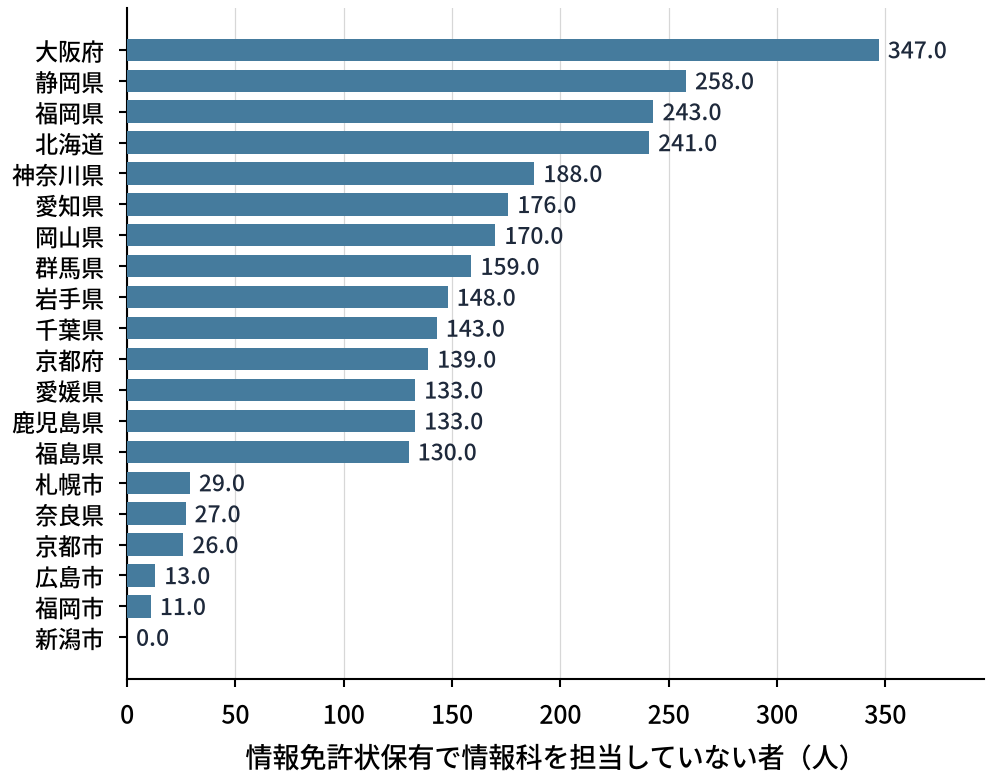
\includegraphics[width=\columnwidth]{chart_japan_high_school_informatics.png}\caption{情報免許状保有で情報科を担当していない者の値の比較（上位・下位と日本を抜粋）．赤が日本}\end{figure}
\begin{figure}[t]\centering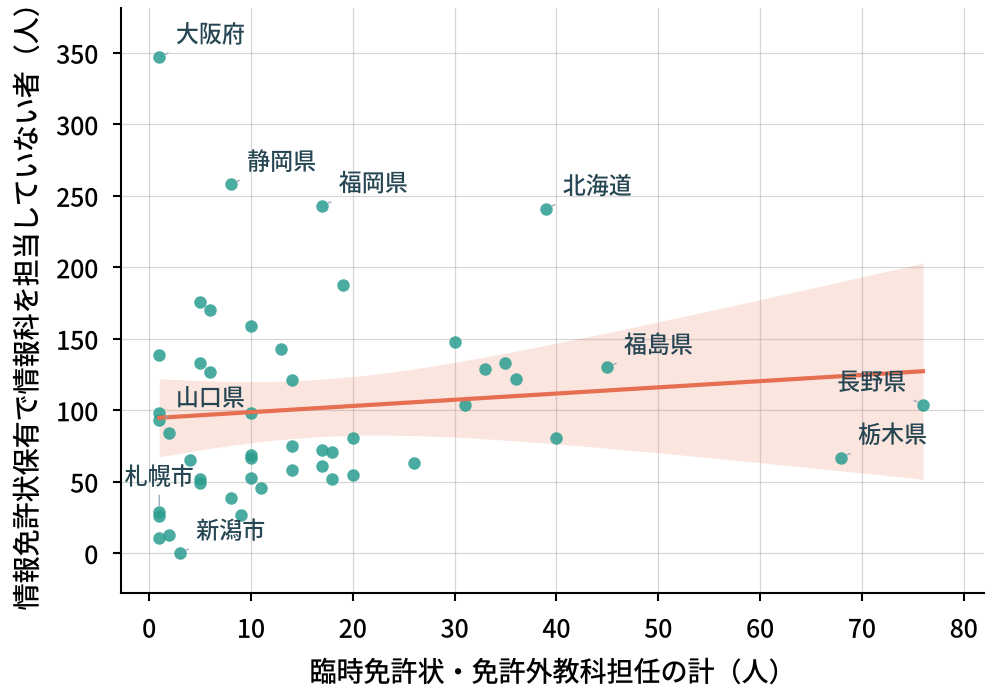
\includegraphics[width=\columnwidth]{chart_secondary_japan_high_school_informatics.png}\caption{臨時免許状・免許外教科担任の計と情報免許状保有で情報科を担当していない者の関連（回帰直線と，その平均の95\%信頼区間の帯，n=49）}\end{figure}
\section{考察}
RQ1とRQ2の結果をまとめると，免許状のない担当者は少数の自治体に集中し，臨時免許状と免許外教科担任の使い分けは自治体によって異なっていた．また，免許状のない担当者の人数と，免許状を持つが担当していない者の人数との間に，関連は見られなかった．免許状のない担当者が多い自治体で，免許状を持つが担当していない者が少ないわけではなく，その逆でもない．ただし，人数は実数で，規模の大きい自治体ほど免許状保有者が多くなりうる．高校数や教員数で割ると，結果が変わる可能性がある．また，49自治体では，検出力80\%で見つけられる相関は\textit{r}=.39程度以上であり，それより小さい関連の有無は，このデータでは判断できない．順位相関では\textit{ρ}=.24（\textit{p}=.09）と，弱い正の関連がうかがえるが，有意ではなかった．

この結果から，免許状のない担当者の多さと，免許状を持つが担当していない者の多さが，自治体の間で同じ向きに並ぶとは言えない．人数が実数で自治体の規模を含むため，その理由や免許状保有者の不足との関係は，本研究のデータでは分からない．しかし，その理由は本研究のデータでは分からない．免許状を持つが担当していない者の多くは，他の教科の免許状も持ち，その教科を担当している可能性がある．その場合，担当していないことは配置の不備ではなく，通常の姿である．情報科を担当できる状況にあるのかも，資料に示されていない．教員の資格と担当教科の不一致は，Ingersoll (1999) が米国の中等学校で示したように，他の国でも見られる．専門性を教科内容の知識（Shulman，1986）や，教科・教授法・技術の統合（Mishra and Koehler，2006）として捉えると，免許状は専門性の制度的な目印の一つにすぎない．免許状のない担当者が，どのような専門性を持ち，どのような支援を受けているかは，本データからは分からない．

令和5年4月の見込みでは，80人が7自治体に残るとされているが，これは計画にもとづく値であり，実現したかは本研究では確認していない．世界的に見ても，情報科の教員の養成と配置は共通の課題とされており（Hubwieser et al.，2015），日本の自治体別の表は，その一端を示すものである．本研究の限界は，(1)人数を規模で割っていないこと，(2)0人の16自治体が表に載っていないこと，(3)令和4年5月1日の1時点であること，(4)授業の質や生徒への影響を扱っていないこと，である．今後は，高校数や教員数で標準化した比率での検討と，免許状を持つが担当していない者の配置の実態に関する調査が必要である．
\section*{参考文献}
\begingroup\scriptsize\raggedright\interlinepenalty=10000 
\begin{list}{}{\setlength{\leftmargin}{1.5\zw}\setlength{\itemindent}{-1.5\zw}\setlength{\labelwidth}{0pt}\setlength{\labelsep}{0pt}\setlength{\itemsep}{1pt}\setlength{\parsep}{0pt}\setlength{\topsep}{0pt}\setlength{\listparindent}{0pt}}
\item HUBWIESER, P., GIANNAKOS, M. N., BERGES, M., BRINDA, T., DIETHELM, I., MAGENHEIM, J., PAL, Y., JACKOVA, J. and JASUTE, E. (2015) A global snapshot of computer science education in K-12 schools. Proceedings of the 2015 ITiCSE on Working Group Reports, 65-83.
\item INGERSOLL, R. M. (1999) The problem of underqualified teachers in American secondary schools. Educational Researcher, \textbf{28} (2) ：26-37.
\item MISHRA, P. and KOEHLER, M. J. (2006) Technological pedagogical content knowledge: A framework for teacher knowledge. Teachers College Record, \textbf{108} (6) ：1017-1054.
\item 文部科学省 (2019) 高等学校学習指導要領（平成30年告示）解説 情報編. 開隆堂出版.
\item 文部科学省 (2022) 高等学校情報科担当教員の配置状況及び指導体制の充実に向けて（令和4年11月）. 文部科学省初等中等教育局学校デジタル化PT.
\item 大学入試センター (2023) 令和7年度大学入学者選抜に係る大学入学共通テスト問題作成方針. 独立行政法人大学入試センター.
\item SHULMAN, L. S. (1986) Those who understand: Knowledge growth in teaching. Educational Researcher, \textbf{15} (2) ：4-14.
\item WING, J. M. (2006) Computational thinking. Communications of the ACM, \textbf{49} (3) ：33-35.
\end{list}\endgroup
\section*{Summary}
{\footnotesize\setlength{\parindent}{0pt}Using the published MEXT tables (November 2022), this study examined whether local governments with more high school informatics teachers who hold only a temporary licence or teach out of field also have more licence holders who do not teach the subject. Nationwide, 796 of 4,756 informatics teachers taught without an informatics licence, while 6,088 of 10,048 licence holders did not teach informatics. Across 49 prefectures and designated cities, the number of teachers without a licence (median 10, maximum 76 in Nagano) was not related to the number of licence holders not teaching (r = .10, BF10 = 0.14), and in 47 local governments the latter exceeded the former. Counts are not scaled by school or teacher numbers, and the reasons and the realisation of the plan for April 2023 cannot be determined from these data.\par\smallskip KEYWORDS: INFORMATICS TEACHERS, TEMPORARY LICENCE, OUT-OF-FIELD TEACHING, TEACHER ASSIGNMENT, PREFECTURAL COMPARISON\par}
\medskip\noindent\fbox{\parbox{\dimexpr\columnwidth-2\fboxsep-2\fboxrule}{\footnotesize\gtfamily 【付記：生成AIによる自動執筆に関する開示】\\ 本論文は学生への教育目的で作成している．使用しているデータは公的オープンデータである．統計の算出はPythonで行い，文章は生成AI（Anthropic Claude等）を活用して作成した．記載した統計数値は元データに準拠しているが，教育学的な考察や提言の妥当性は，指導現場の実情に応じて，批判的に吟味してほしい．}}
\end{document}
